\documentclass[a4paper,11pt,pdf]{pacmanreport}

%%=== Aditional packages


%%=== Local definitions
\graphicspath{{images/}{../shared_images/}}

%% ================================
%% PROJECT INFO 

\project{}
\projectid{FP7-IST-60918}
\projectstart{1 March 2013}
\duration{36}

%% ================================
%% DELIVERABLE INFO 

\title{Planning Active Information Gathering for Haptics and Vision}
\deliverableid{DR 3.2}
\author{C. Zito, ...}
\address{University of Birmingham}
\email{cxz004@cs.bham.ac.uk}
\headertitle{shorted title}
\headerauthor{shortauthor}

\duedate{2015-02-27}
\submissiondate{2015-02-27}
\leadpartner{BHAM}
\revision{draft}
\disseminationlevel{PU}


%% UNCOMMENT: to get the logo; if you've copied this file to a directory yearX/wpY/ then this should work
\reportlogo{pacmanlogo}


\begin{document}

\maketitle

\begin{abstract}
\noindent Here comes the abstract
\end{abstract}


\vspace{.2em}
\hrule

\footnotesize

\tableofcontents

\normalsize

\newpage

\section*{Executive Summary}

What does the report present? What tasks does it address? How has progress been evaluated? What previous reports does this report follow up on? 

\section*{Role of [YOUR TOPIC] in PaCMan}

What role do the tasks addressed in this report play in the larger context of PaCMan? How do these tasks, how does report, contribute to achieving the overall goals for PaCMan? 

\section*{Contribution to the PaCMan scenario}

How do the results presented in this report contribute to the PaCMan\cite{ProjectWebsite} scenarios and prototypes? 


\newpage

\section{Tasks, objectives, results}

\subsection{Planned work}

What tasks was the report supposed to address? What objectives, results were these tasks to achieve? 

\subsection{Actual work performed}

What does the report actually present? How have the tasks been addressed? To what extent have the intended objectives been achieved? Why, how -- or why not? 

\subsection{Relation to the state-of-the-art}

How are the obtained results related to the state-of-the-art? 

\bibliographystyle{ieeetr}
\bibliography{../shared_bibliography/abbreviations,./bibliography/DR32}

\newpage

\appendix
\section{Annexes}

Which papers / articles are included in the report? Mention titles, authors, publication info; abstract; and a one-liner relating the publication back to the discussion on actual work performed. 

% template for annexes
\subsection{Book chapter/Article/Technical Report: \em TITLE}
\begin{description}
    \item[Authors] 
    \item[Info] % UNDER REVIEW / IN PRESS / ACCEPTED FOR PUBLICATION (PROVIDE WHERE) / PUBLISHED AND AVAILABLE ONLINE (PROVIDE DOI)
    \item[Abstract]
    \item [Relation with the deliverable] 
    \item[Attachment] %if so, e.g. (following pages until next annex) or The article can be downloaded at the DOI link above, hence no attachment is provided
\end{description}
% attach your PDF(s) if required, pusblished and online available documents do not require it if you provide the doi (only doi are permitted)
%\includepdf[pages=-]{./attachedPapers/YOURFILE.pdf

\subsection{Technical Report: \em The Next Best Touch or Non-Touch:
Object Pose Estimation via Sculpting with Compliant Hands}
\begin{description}
    \item[Authors] Alexander Rietzler, Carlos J. Rosales, Marco Gabiccini, Justus Piater
    \item[Info] Paper Draft% UNDER REVIEW / IN PRESS / ACCEPTED FOR PUBLICATION (PROVIDE WHERE) / PUBLISHED AND AVAILABLE ONLINE (PROVIDE DOI)
    \item[Abstract] Many robotic tasks rely on the ability of a vision system to accurately estimate the 6 dimensional pose of objects in a scene.
In many cases a single vision sensor does not provide sufficient information to discriminate a single correct
pose of an object. 
This paper solves the problem of refining the pose distribution 
of an object solely via proprioceptive sensing of occupancy.
Our main novel contribution is an algorithm that plans a robot arm-hand trajectory such that 
information gathered about the object pose belief is maximized while at the same time impact on the object is minimized. 
This may result in actions that do not make contact with the object at all.
Impact on the object is further reduced by using a compliant robotic hand.
    \item [Relation with the deliverable] This report reports work done under\\ Task~2.3 by introducing a method for reducing an object's pose uncertainty by performing proprioceptive information
    gathering actions.
    \item[Attachment] (following pages) %if so, e.g. (following pages until next annex) or The article can be downloaded at the DOI link above, hence no attachment is provided
\end{description}
% attach your PDF(s) if required, pusblished and online available documents do not require it if you provide the doi (only doi are permitted)
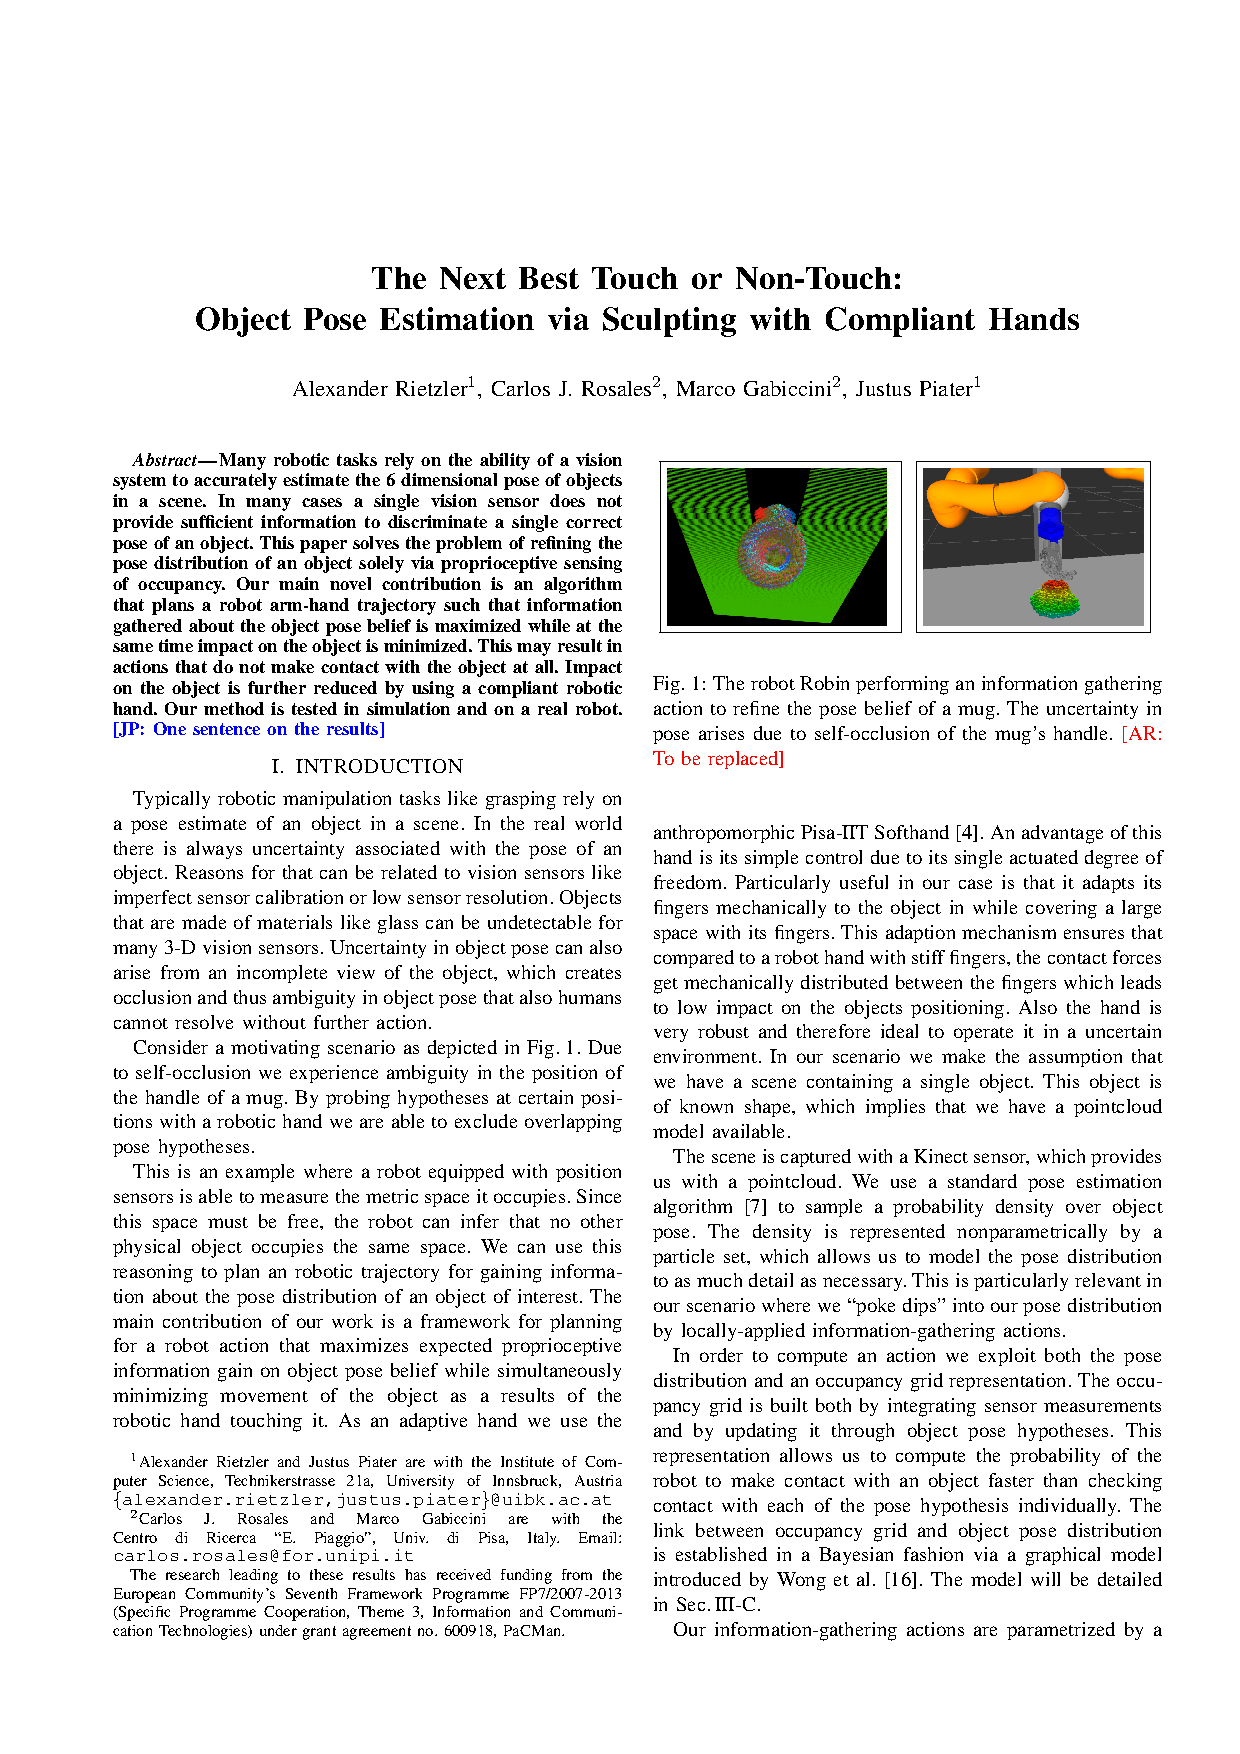
\includepdf[pages=-]{./attachedPapers/iros_draft_rietzleretal.pdf}


\end{document}
